% Study article in SBPO-like layout (A4, Times 12pt, unnumbered title block, Resumo + Abstract).
% Figures are referenced from the stage folders of this repository; compile from the repo root.
\documentclass[12pt,a4paper]{article}

\usepackage[utf8]{inputenc}
\usepackage[T1]{fontenc}
\usepackage[english]{babel}
\usepackage{mathptmx}
\usepackage[top=3cm,bottom=2cm,left=3cm,right=2cm]{geometry}
\usepackage{graphicx}
\usepackage{booktabs}
\usepackage{amsmath,amssymb}
\usepackage{caption}
\usepackage{float}
\usepackage{titlesec}
\usepackage[hidelinks]{hyperref}

\captionsetup{font=small,labelfont=bf}
\titleformat{\section}{\normalsize\bfseries\MakeUppercase}{\thesection.}{0.5em}{}
\titleformat{\subsection}{\normalsize\bfseries}{\thesubsection.}{0.5em}{}
\setlength{\parskip}{4pt}

\graphicspath{
  {../ANALISE_EXPLORATORIA_2_ETAPA/resultados_scripts/}
  {../MODELAGEM_AVALIACAO_3_ETAPA/resultados_scripts/}
}

\begin{document}

\begin{center}
{\large\bfseries COHERENT AND NON-NEGATIVE HIERARCHICAL FORECASTING OF RSV-ASSOCIATED HOSPITALIZATIONS IN CHILDREN UNDER TWO IN BRAZIL}

\vspace{0.8cm}
Thiago Paes, Joan Souza, Matheus Accioly, Isabelle Gagno\\
Pontifícia Universidade Católica do Rio de Janeiro (PUC-Rio)\\
IND2616 -- Time Series
\end{center}

\vspace{0.5cm}
\noindent\textbf{RESUMO}

\noindent Este trabalho prevê o número semanal de internações por SRAG associada ao vírus sincicial respiratório (VSR) em crianças menores de dois anos, nos níveis UF, região e Brasil. A partir de 4,68 milhões de notificações do SIVEP-Gripe (2019--2026), obteve-se um painel de 33 séries e 395 semanas maduras. Modelos de referência, ETS e SARIMA(X) foram comparados em validação temporal expansiva com 58 origens e horizontes de 1 a 13 semanas, e seis estratégias de reconciliação hierárquica foram avaliadas. A política final usa MinT com restrição de não negatividade em 1 e 4 semanas e o ingênuo sazonal em 8 e 13 semanas, garantindo previsões coerentes e sem contagens negativas.

\noindent\textbf{PALAVRAS CHAVE.} Previsão hierárquica. Reconciliação MinT. Vigilância epidemiológica.

\noindent\textbf{Tópicos:} EST -- Estatística; SA -- PO na Área de Saúde.

\vspace{0.3cm}
\noindent\textbf{ABSTRACT}

\noindent This work forecasts the weekly number of severe acute respiratory illness (SARI) hospitalizations associated with respiratory syncytial virus (RSV) in children under two years old, at state (UF), regional and national levels. From 4.68 million SIVEP-Gripe notifications (2019--2026), a panel of 33 series and 395 mature weeks was built. Benchmark, ETS and SARIMA(X) models were compared in an expanding-window temporal validation with 58 origins and horizons of 1 to 13 weeks, and six hierarchical reconciliation strategies were evaluated. The final policy applies non-negative MinT at 1 and 4 weeks and the seasonal naive at 8 and 13 weeks, yielding coherent forecasts with no negative counts.

\noindent\textbf{KEYWORDS.} Hierarchical forecasting. MinT reconciliation. Epidemiological surveillance.

\noindent\textbf{Paper topics:} EST -- Statistics; SA -- OR in Health.

\newpage
%=====================================================================
\section{Introduction}

Respiratory syncytial virus (RSV) is a major cause of severe respiratory disease in infants and drives a seasonal surge in pediatric hospital demand. In Brazil this surge is neither simultaneous nor equally intense across the territory: a single national forecast hides local pressure, while independent state forecasts typically do not add up to the regional or national totals. A health manager who reads three inconsistent numbers for the same week cannot act on them jointly.

The guiding question of this study is:

\begin{quote}
\emph{Is it possible to forecast, 1 to 13 weeks ahead, the weekly number of RSV-associated SARI hospitalizations in children under two, while keeping the forecasts coherent across state, region and country?}
\end{quote}

The contribution is not a single best model, but a \emph{forecasting policy}: a rule, chosen by horizon, that (i) is validated without temporal leakage, (ii) beats or matches simple benchmarks, (iii) makes the 27 states sum exactly to their 5 regions and to Brazil, and (iv) never produces negative counts. The target is the series of notified, laboratory-confirmed hospitalizations; it is not an estimate of total community RSV incidence.

The paper is organized as follows. Section~\ref{sec:data} defines the data and the outcome; Section~\ref{sec:eda} summarizes the exploratory findings that shaped the modeling; Section~\ref{sec:method} describes the evaluation design, the models and the reconciliation methods; Section~\ref{sec:results} reports the results; Section~\ref{sec:op} applies the policy to the latest data; and Section~\ref{sec:conc} concludes.

%=====================================================================
\section{Data and Outcome Definition}\label{sec:data}

\subsection{Source}
The primary source is the SIVEP-Gripe SARI microdata (2019--2026) published by OpenDataSUS. Eight annual Parquet files (333.67\,MB, 4{,}678{,}812 raw notifications, 194 fields common to all years) were \emph{frozen} and verified by URL, size and SHA-256 hash, so that the analysis refers to an identifiable version of a dataset that is periodically republished.

\subsection{Case definition}
A record enters the study when all conditions hold: valid symptom-onset date; age between 0 and 24 months (exclusive); valid state of residence; hospitalization recorded; and RSV confirmed by PCR \emph{or} antigen test. Missing tests were never interpreted as negative results. The data treatment chain is summarized in Table~\ref{tab:treat}.

\begin{table}[H]
\centering\small
\caption{Data treatment decisions.}\label{tab:treat}
\begin{tabular}{p{2.6cm}p{5.2cm}p{6.2cm}}
\toprule
Step & Decision & Rationale / result \\
\midrule
Source & Freeze 8 official files & Exact reproducibility. \\
Structure & Inventory all 194 columns & Fields chosen by meaning, not by acronym. \\
Time axis & Symptom-onset date & Complete, closest to epidemiological onset. \\
Geography & State of residence & High completeness. \\
Confirmation & PCR $\cup$ antigen & No lost confirmations, no double counting. \\
Duplicates & Deterministic tie-break rule & 2 duplicated notifications; 2 rows removed. \\
Reporting delay & Flag maturity, keep recent weeks & Separates observed from consolidated data. \\
\bottomrule
\end{tabular}
\end{table}

The final individual-level base contains \textbf{158{,}358} eligible notifications, aggregated by epidemiological week into a panel of 33 geographic nodes (27 states, 5 regions, Brazil) $\times$ 407 weeks (30/12/2018 to 11/10/2026). In closed weeks the sum of states equals Brazil exactly.

\subsection{Data maturity}
Recent counts are incomplete because notifications and lab results arrive late. The annual median delay between onset and availability ranged from 8 to 13 days, and the largest annual 95th percentile reached 86 days (2021). A week was therefore considered \emph{mature} if it was closed and at least 13 weeks older than the source cutoff (19/10/2026). Only the 395 mature weeks (up to 19/07/2026) were used for training and evaluation; the 12 most recent weeks were neither discarded nor treated as zeros, simply not used as targets.

%=====================================================================
\section{Exploratory Analysis}\label{sec:eda}

\textbf{Seasonality with variable level.} Brazil and all regions show a clear annual cycle (Figures~\ref{fig:br} and \ref{fig:saz}). National peaks occurred between epidemiological weeks 11 and 19 (roughly March--May). The Southeast and Center-West peak earlier and more sharply; the Northeast peaked later in recent years; North and South vary more in timing. The level, however, is far from stationary: the national season total went from 5{,}029 (2019) to 1{,}120 (2020), 11{,}124 (2021), 14{,}969 (2022) and 43{,}152 (2025). The pandemic years were kept in the history and not given a causal interpretation, since circulation, testing and reporting all changed.

\begin{figure}[H]
\centering
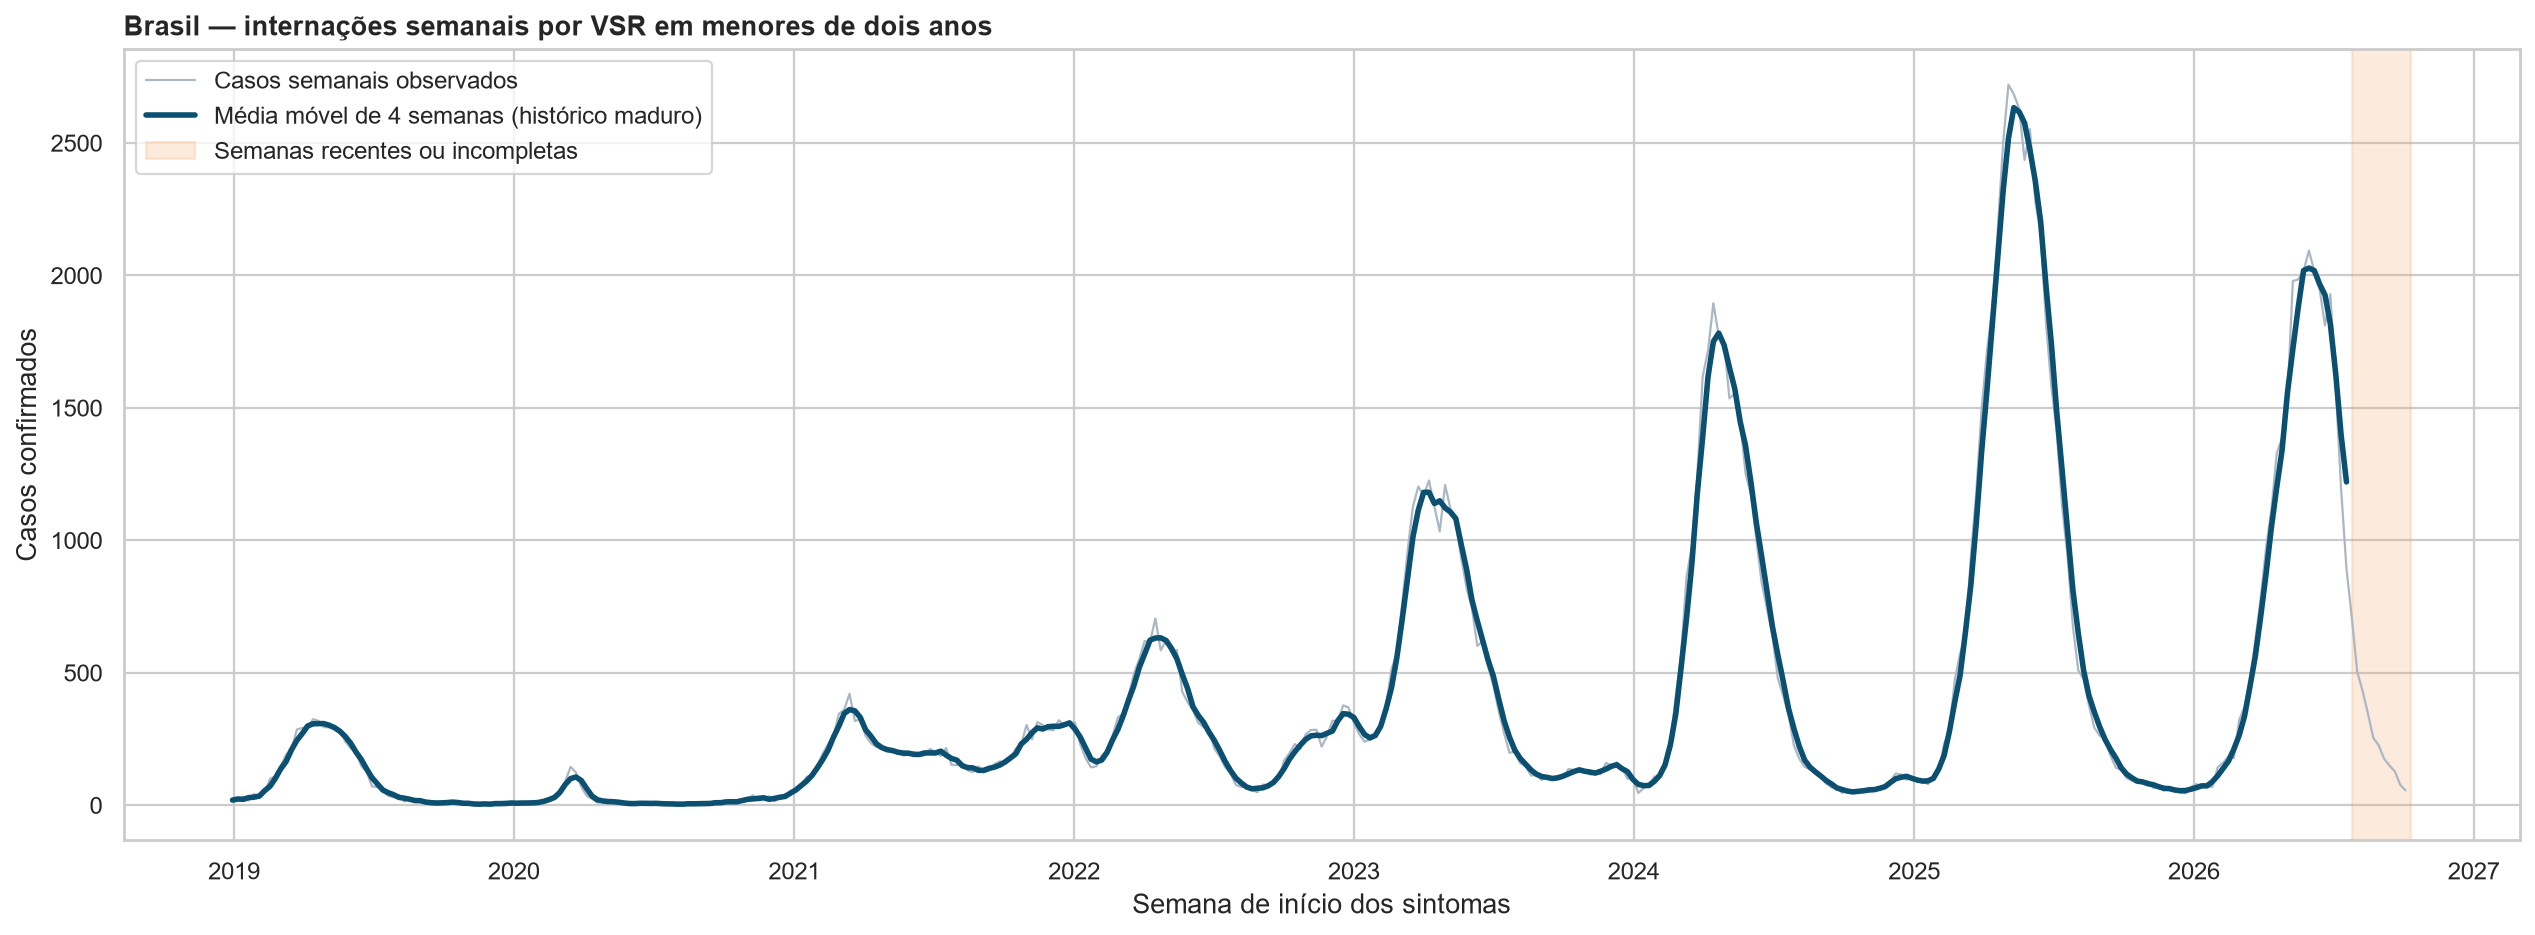
\includegraphics[width=\textwidth]{etapa_13_series_brasil_regioes/serie_temporal_brasil.png}
\caption{Weekly RSV-associated SARI hospitalizations, children under two, Brazil.}\label{fig:br}
\end{figure}

\begin{figure}[H]
\centering
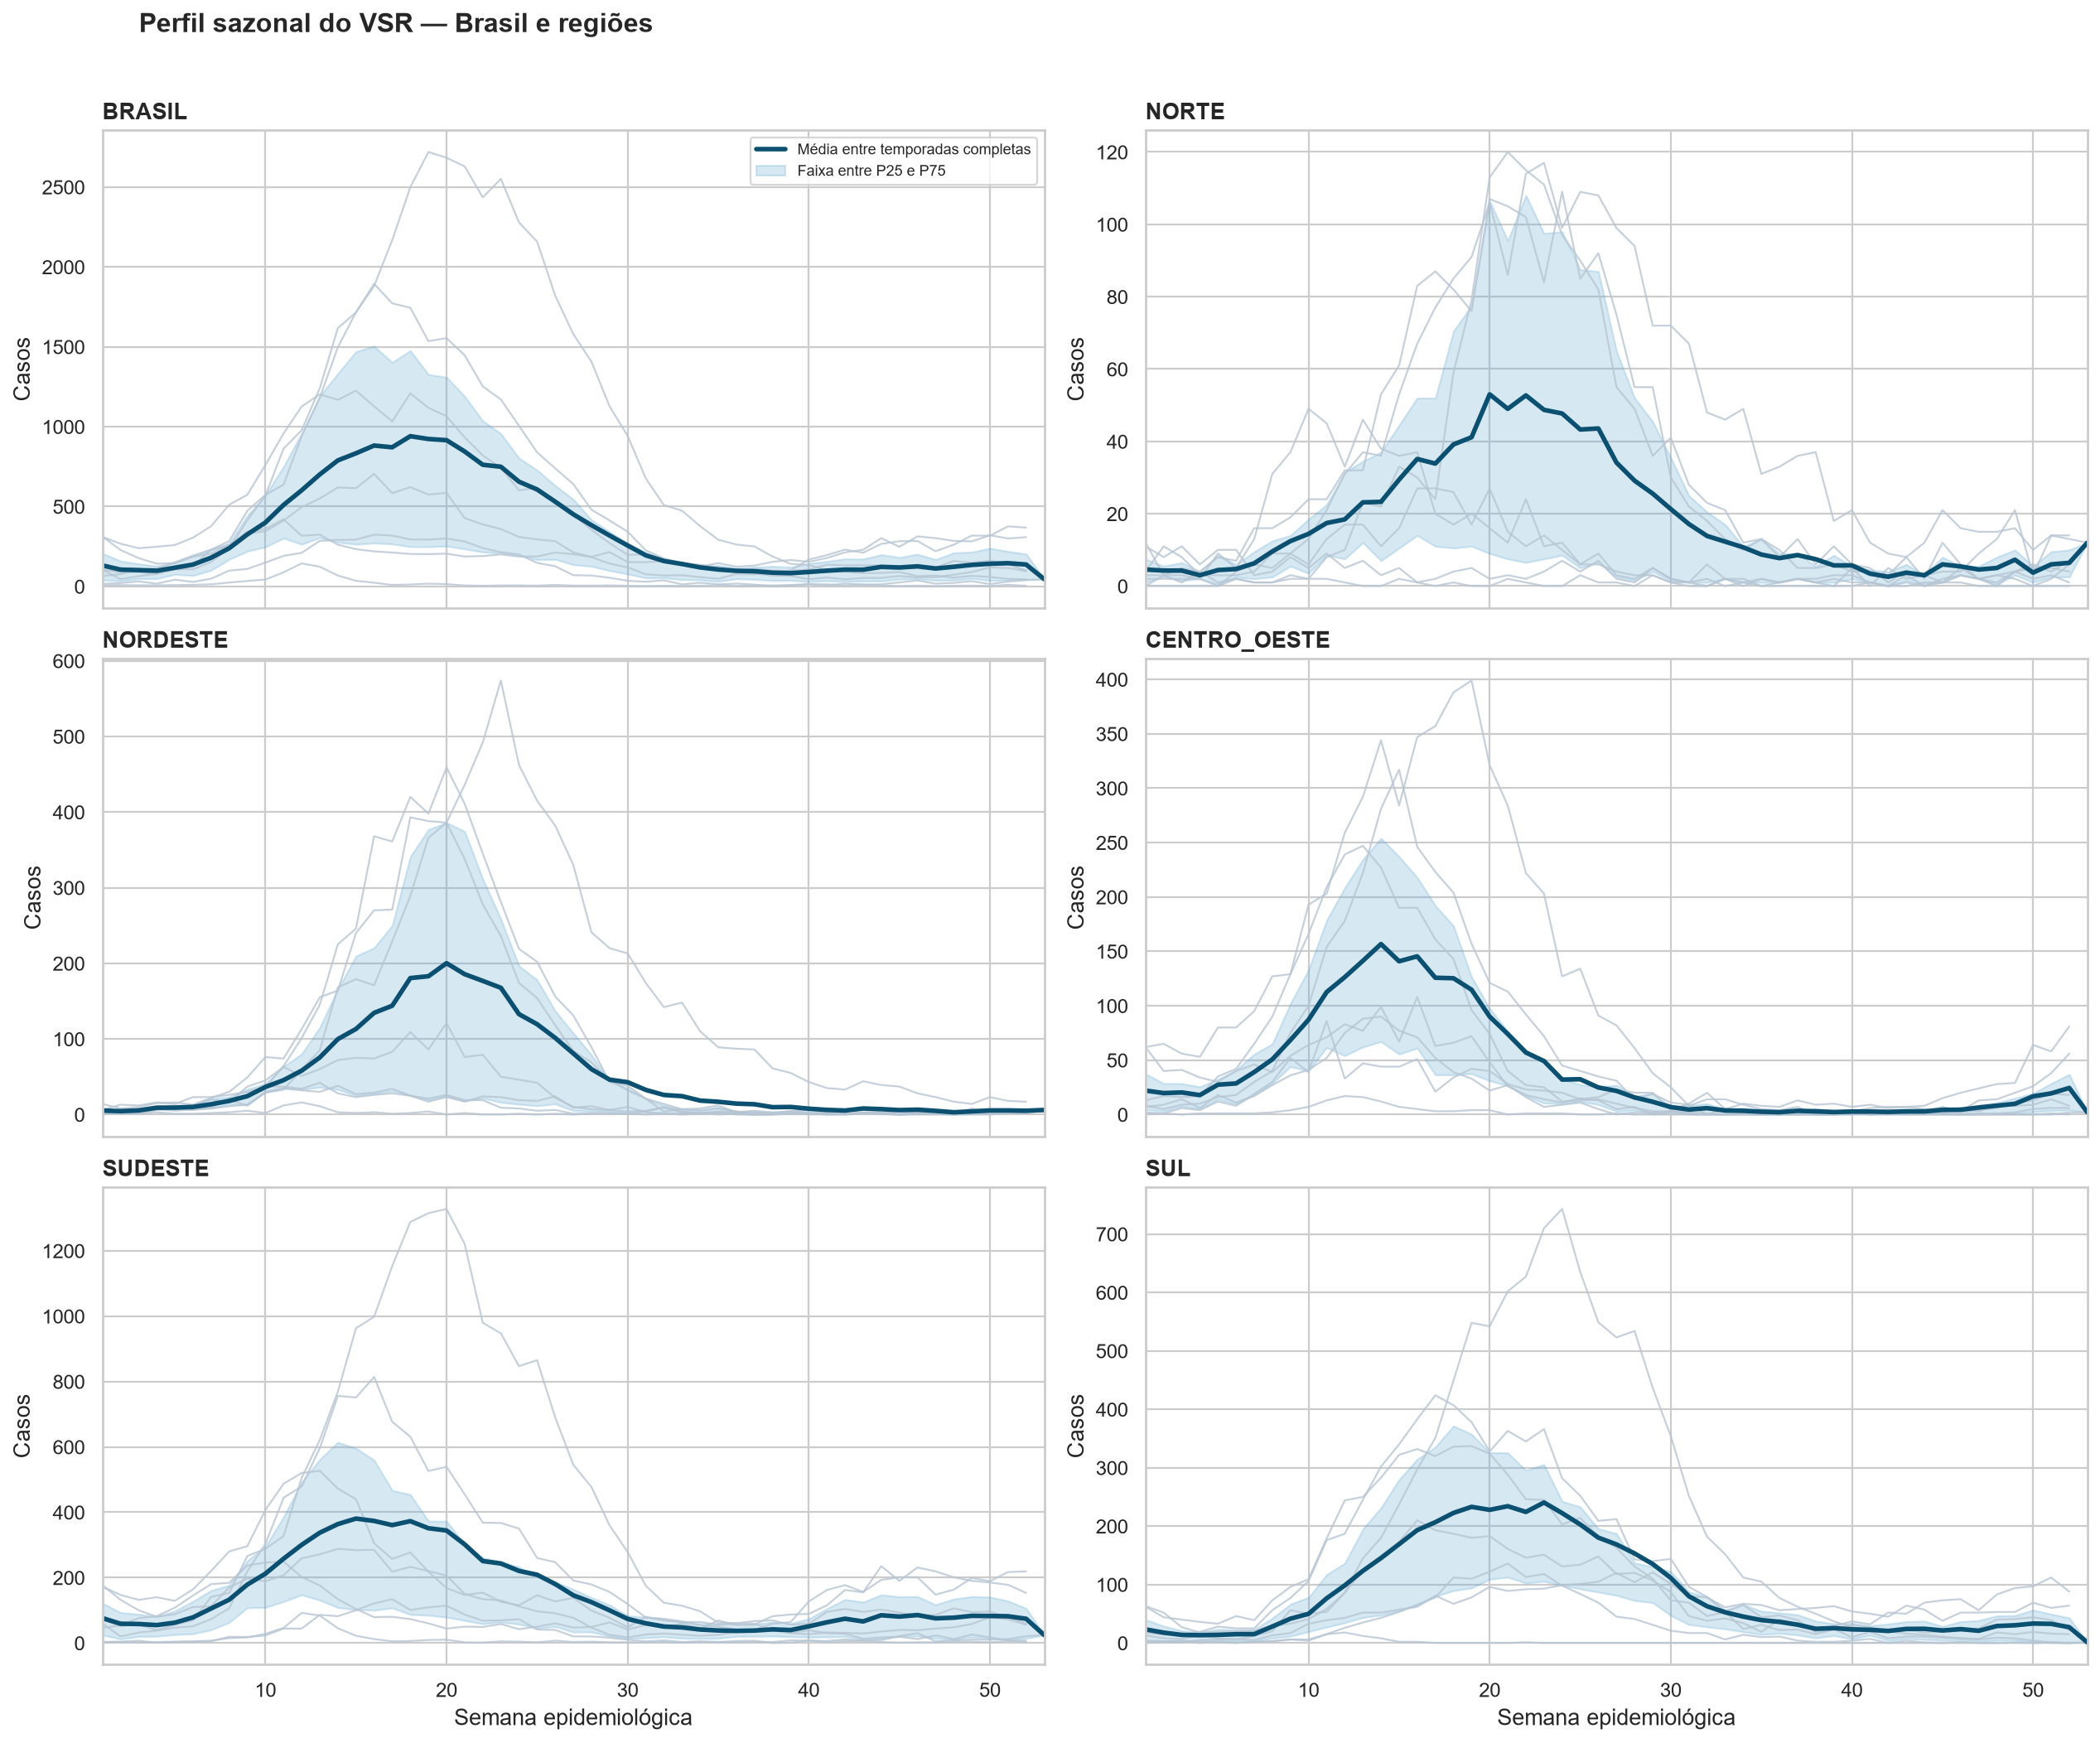
\includegraphics[width=\textwidth]{etapa_14_sazonalidade/sazonalidade_brasil_regioes.png}
\caption{Seasonal profile by epidemiological week, Brazil and regions.}\label{fig:saz}
\end{figure}

\textbf{Strong temporal dependence.} The lag-1 autocorrelation is 0.987 for Brazil and 0.965--0.983 for the regions; at the annual lags 52 and 53 it remains high for Brazil (0.845 and 0.874), supporting both persistence-based and seasonal models (Figure~\ref{fig:acf}).

\begin{figure}[H]
\centering
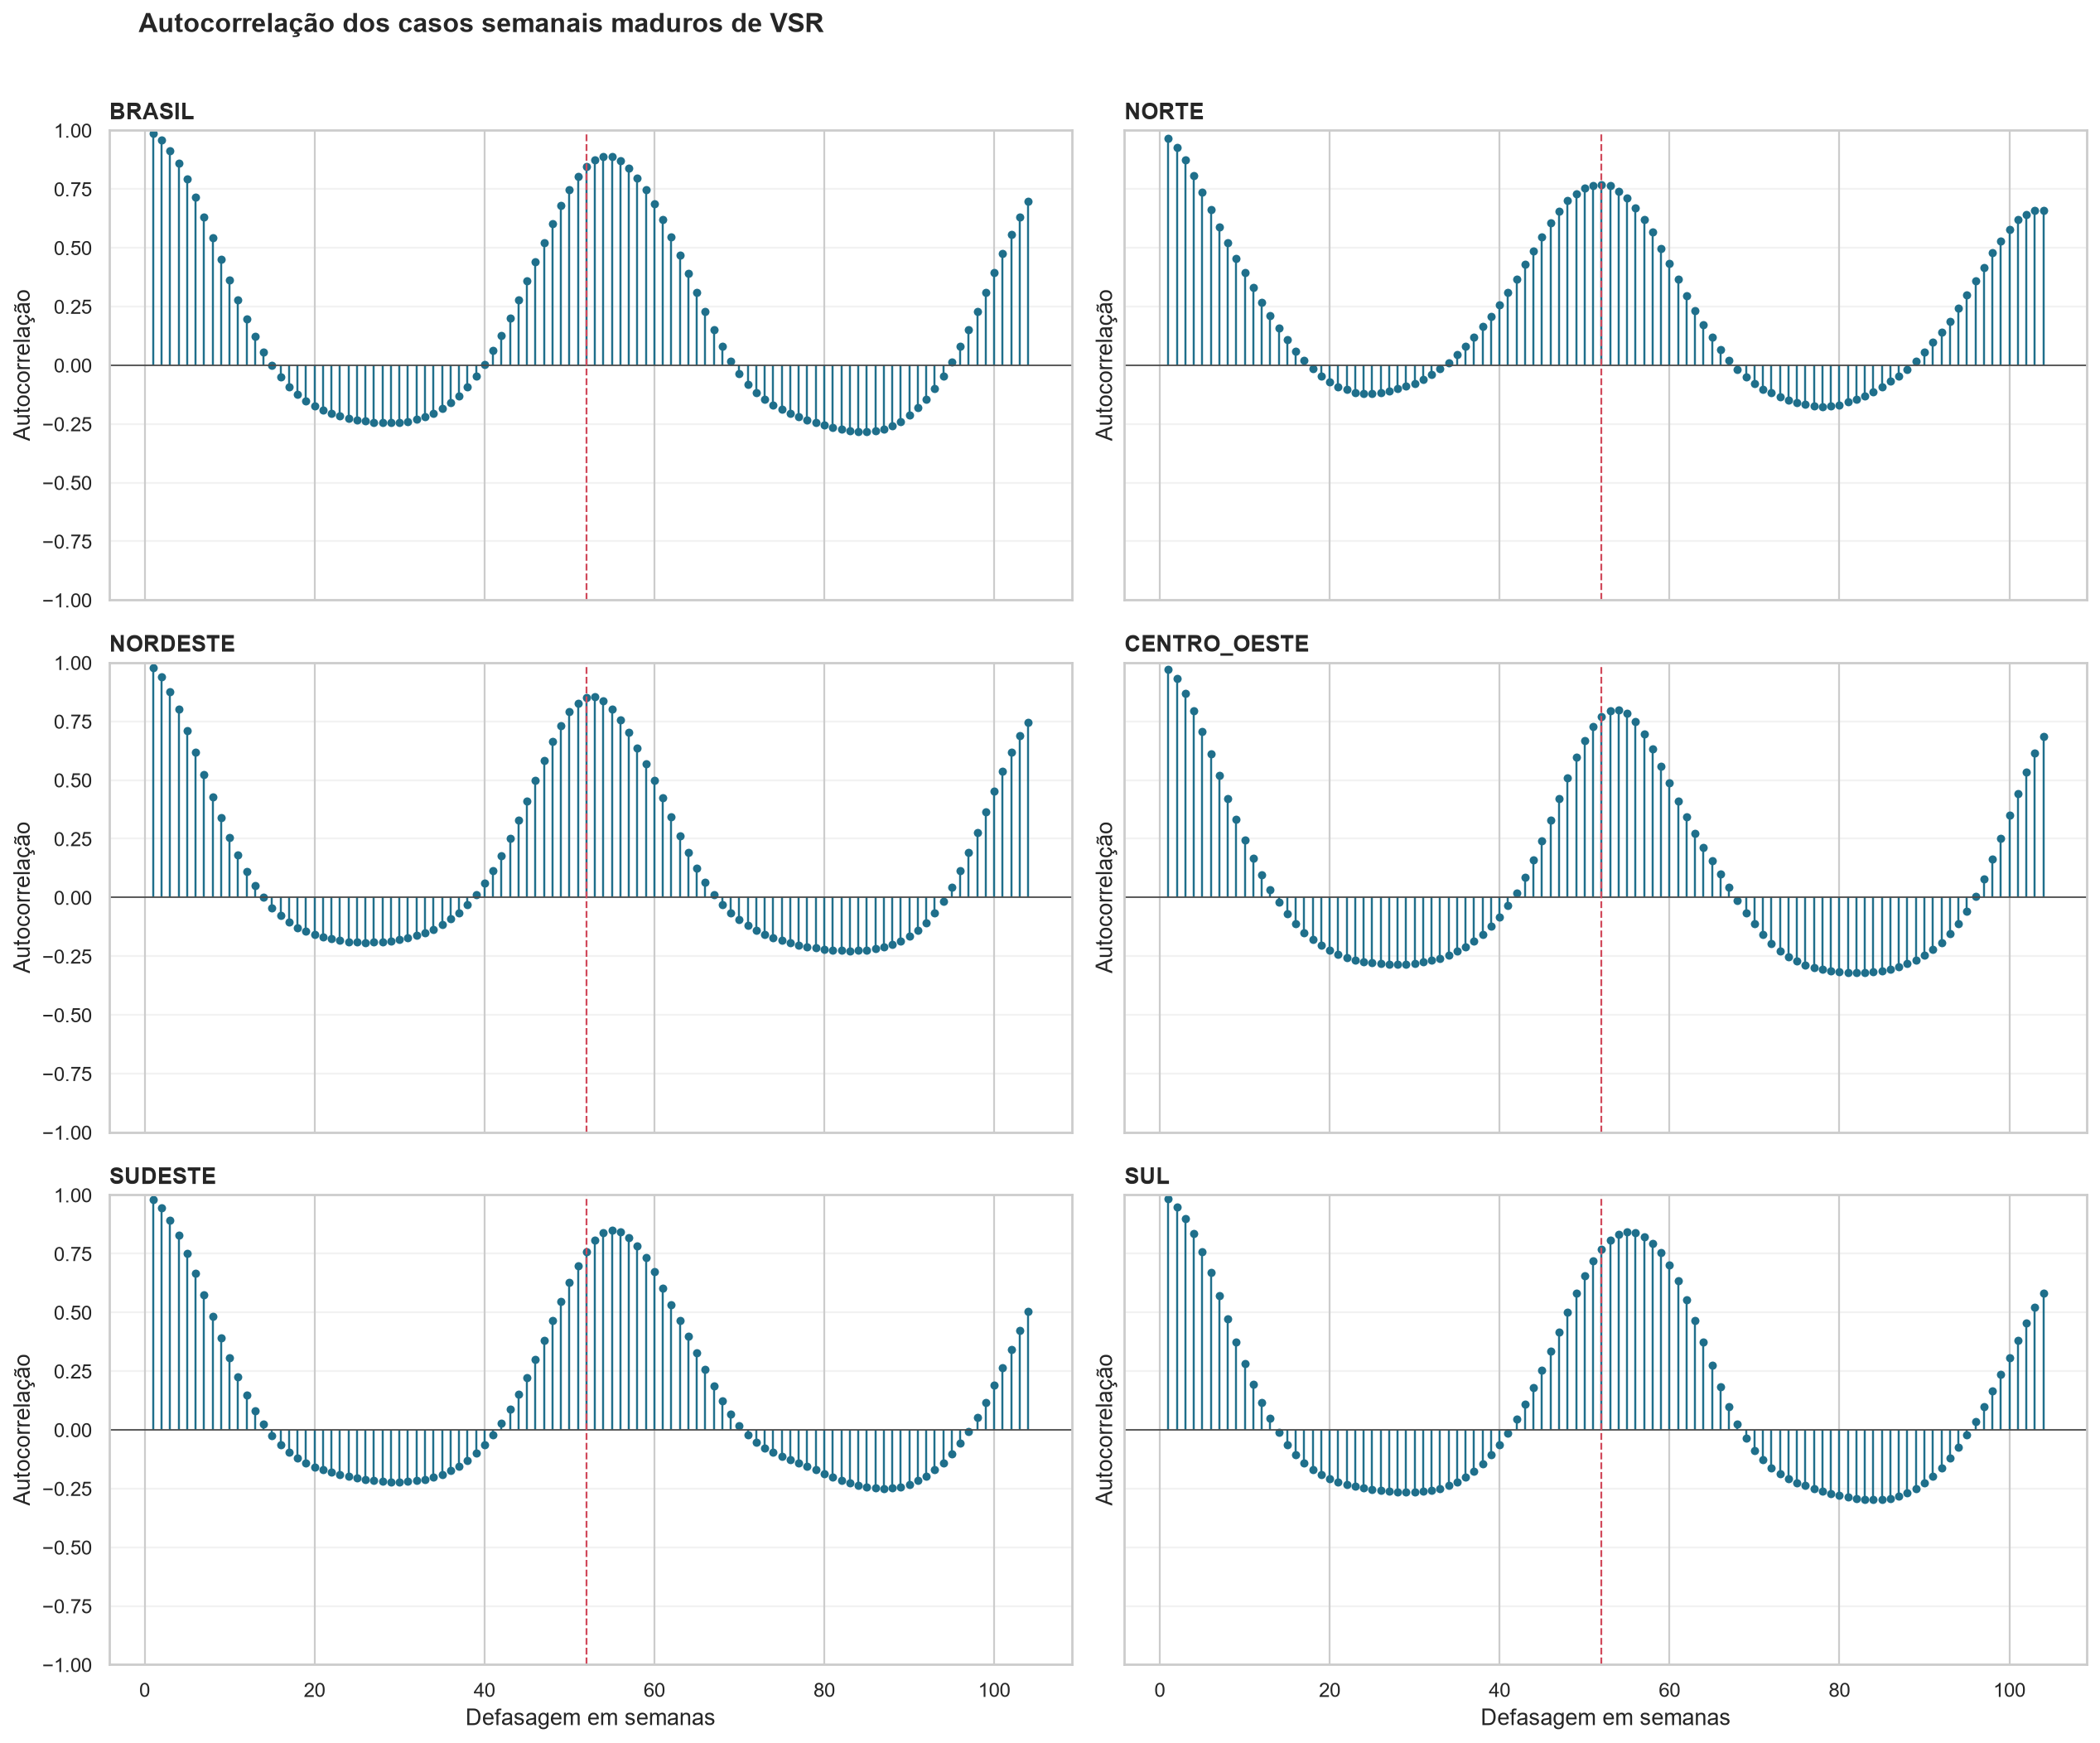
\includegraphics[width=\textwidth]{etapa_17_autocorrelacao/acf_brasil_regioes.png}
\caption{Sample autocorrelation functions, Brazil and regions.}\label{fig:acf}
\end{figure}

\textbf{Heterogeneity and intermittency at state level.} The Southeast concentrates 42.9\% of mature cases and the North 5.5\%. Thirteen states have more than half of their mature weeks with zero cases (Piauí, Mato Grosso, Tocantins and Alagoas exceed 70\%), whereas São Paulo has only 3.0\% (Figure~\ref{fig:uf}). This is the decisive finding for modeling: dense aggregate series and sparse state series call for different forecasting rules.

\begin{figure}[H]
\centering
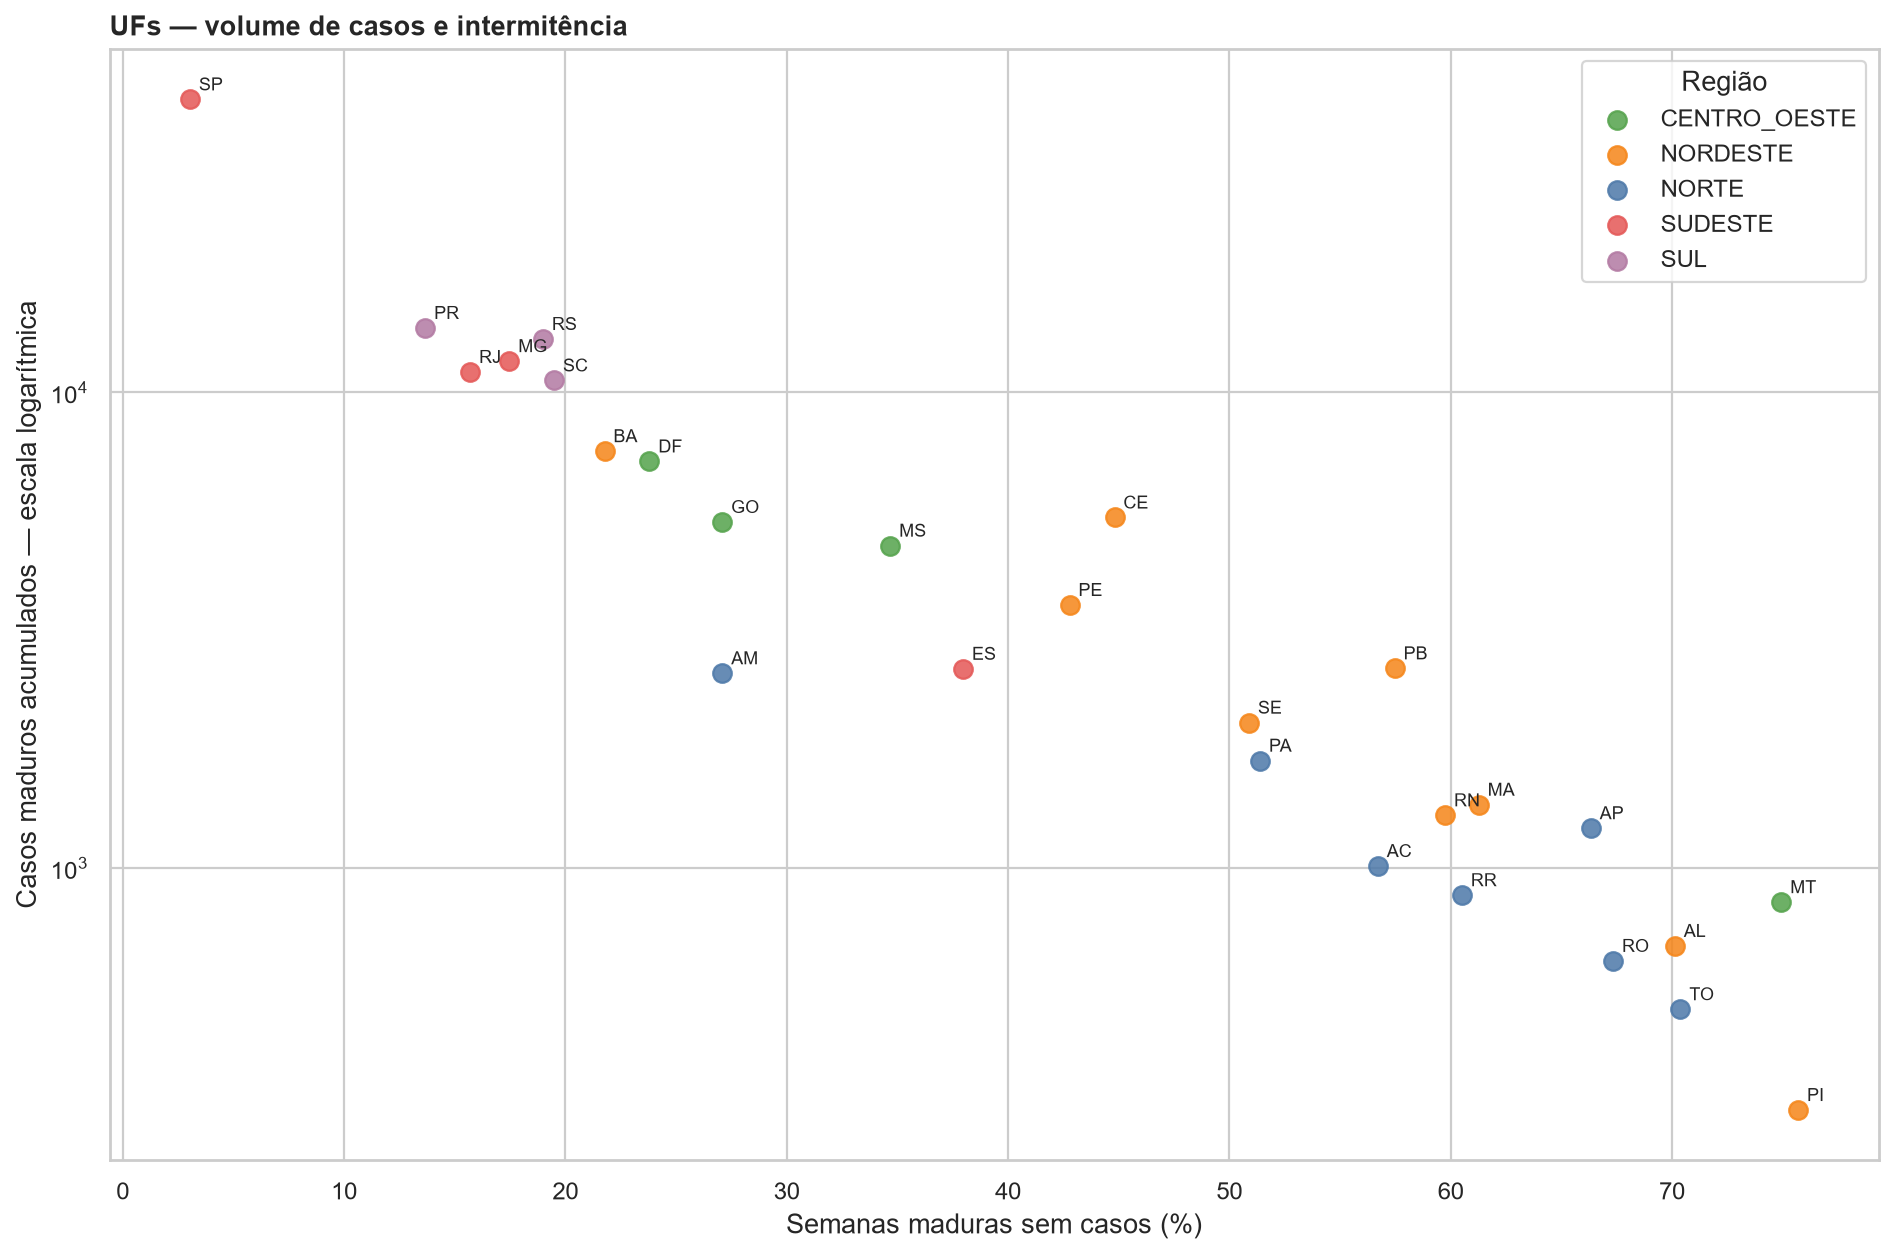
\includegraphics[width=0.95\textwidth]{etapa_15_ufs_intermitencia/ufs_volume_intermitencia.png}
\caption{Case volume versus share of zero weeks by state.}\label{fig:uf}
\end{figure}

%=====================================================================
\section{Methodology}\label{sec:method}

\subsection{Temporal validation design}
Models were compared through expanding-window (rolling-origin) evaluation: each forecast uses only information available at its origin. There are 58 origins per series, starting with at least 156 weeks of history and moving forward every 4 weeks up to 19/04/2026 (Figure~\ref{fig:cal}). Four horizons reflect planning needs: $h=1$ (immediate monitoring), $h=4$ (monthly), $h=8$ (two months) and $h=13$ (one quarter). For Brazil and regions each model yields $6\times58\times4=1{,}392$ forecasts; for the full hierarchy each strategy yields $33\times58\times4=7{,}656$.

\begin{figure}[H]
\centering
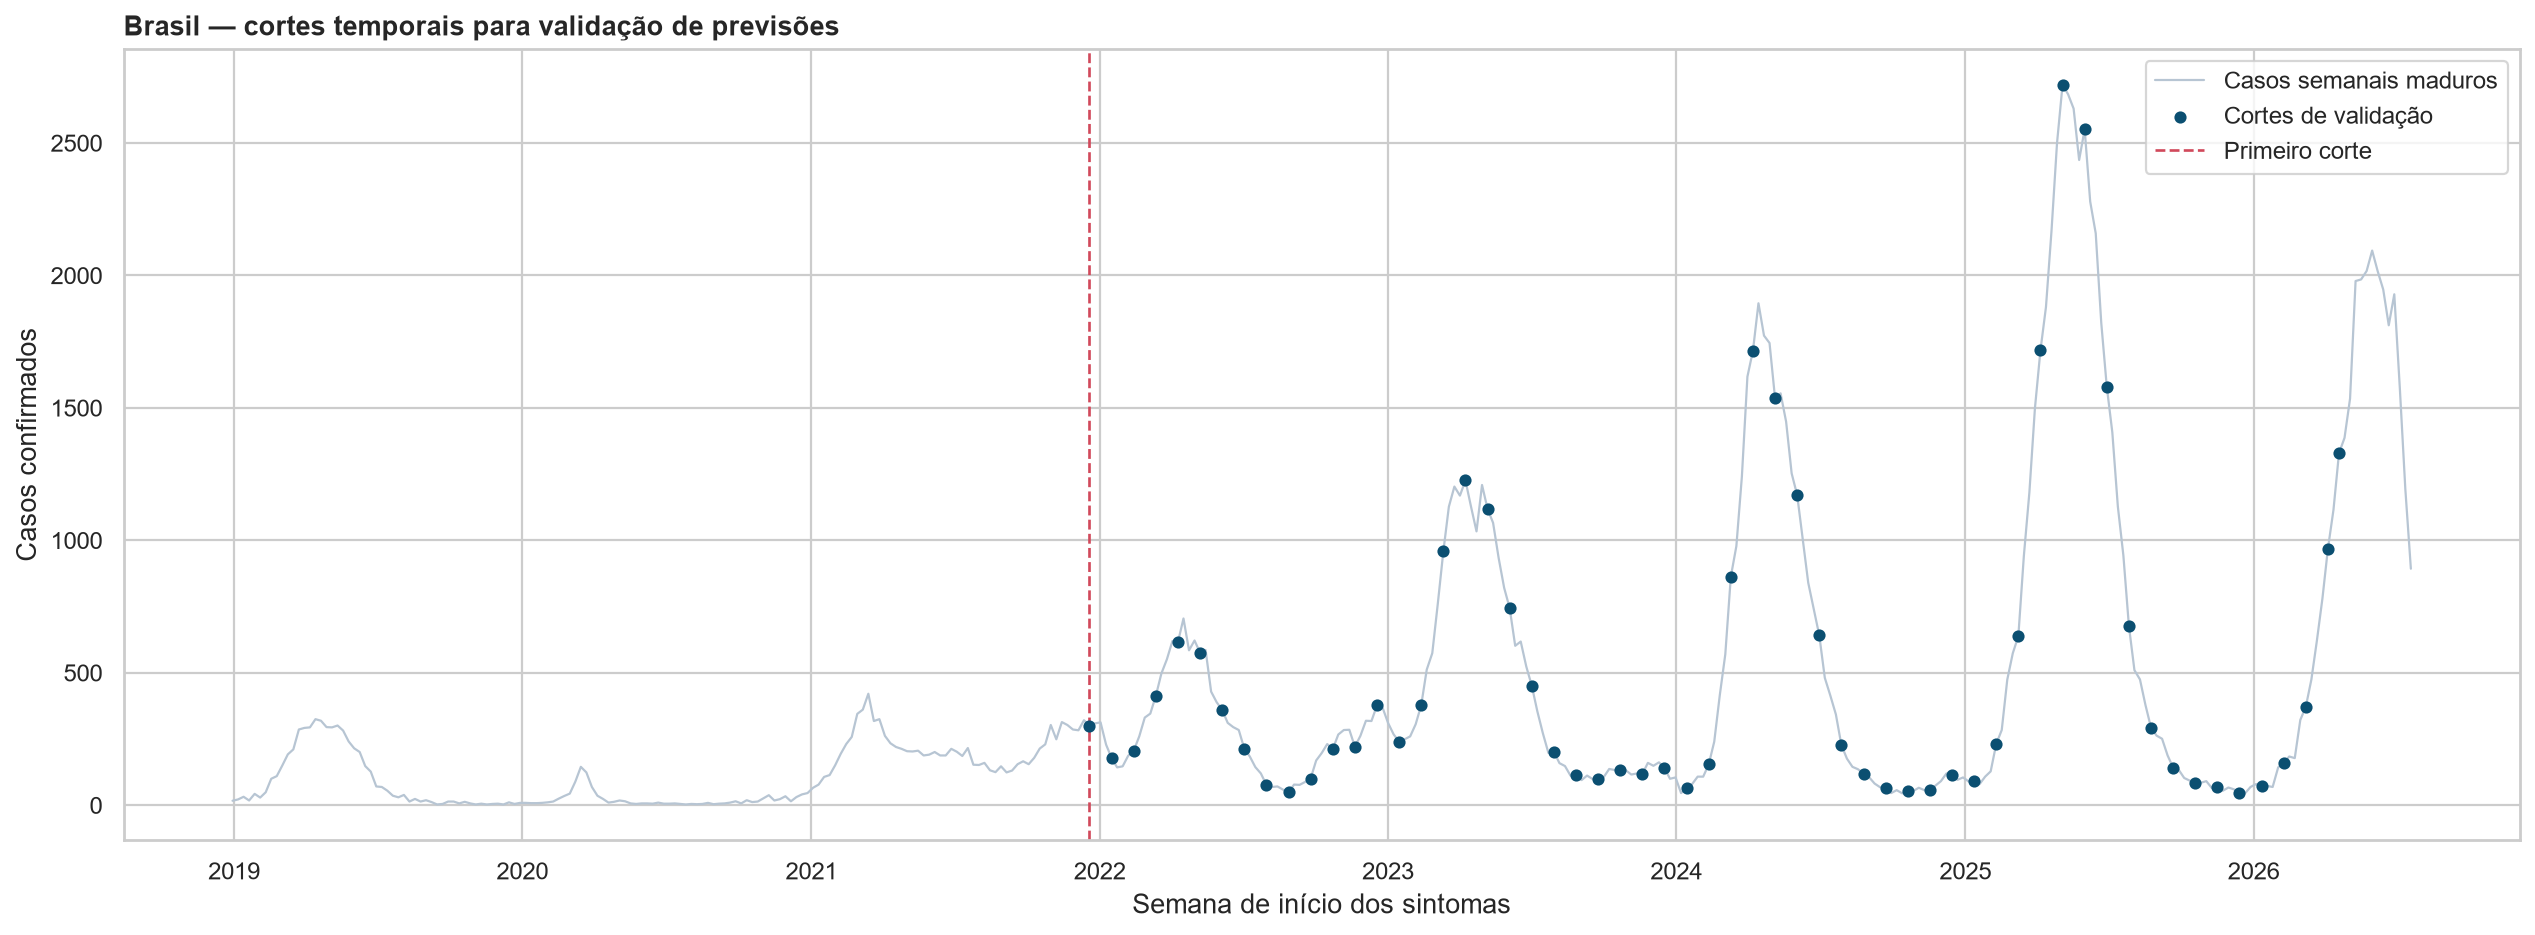
\includegraphics[width=\textwidth]{etapa_19_validacao_temporal/calendario_validacao_brasil.png}
\caption{Rolling-origin validation calendar over the national series.}\label{fig:cal}
\end{figure}

Accuracy was measured by MAE, RMSE and MASE. MAE and RMSE are in cases; MASE divides the absolute error by a seasonal scale, the mean absolute error of the seasonal naive within the training window of each origin, $\mathrm{MASE}=|y_{t+h}-\hat y_{t+h}|\,/\,q_o$ with $q_o=\operatorname{mean}_{t\le o}|y_t-y_{t-52}|$. It is computed with data available up to the origin only (348 scales for Brazil and regions, all positive), making series with very different volumes comparable. A MASE below 1 means the forecast error is smaller than the typical year-over-year change of the series. A model was eligible for ranking only with full coverage (all origins and horizons), no impossible values and, at the hierarchical stage, coherence.

\subsection{Individual (non-hierarchical) models}
\begin{itemize}\setlength\itemsep{0pt}
\item \textbf{Naive}: $\hat y_{t+h}=y_t$.
\item \textbf{Seasonal naive}: $\hat y_{t+h}=y_{t+h-52k}$, the value one season earlier.
\item \textbf{ETS}: additive seasonal ($m=52$), with additive trend and with damped additive trend. Default initialization failed to converge frequently; a robust heuristic initialization was adopted, after which all 348 expected fits converged.
\item \textbf{SARIMA}: two classical seasonal specifications.
\item \textbf{SARIMAX harmonic}: ARMA(1,1) on $\log(1+y)$ with 2 Fourier pairs of period $52.18$ weeks as regressors, a more stable way to represent the annual cycle.
\end{itemize}

\subsection{Hierarchical structure and base forecasts}
Let $\mathbf{b}_t\in\mathbb{R}^{27}$ be the state series and $\mathbf{y}_t=\mathbf{S}\mathbf{b}_t\in\mathbb{R}^{33}$ the full hierarchy, where the summing matrix $\mathbf{S}$ stacks a row of ones (Brazil), five regional indicator rows and $\mathbf{I}_{27}$. A set of independent base forecasts $\hat{\mathbf{y}}_h$ is \emph{coherent} if $\hat{\mathbf{y}}_h=\mathbf{S}\hat{\mathbf{b}}_h$ for some $\hat{\mathbf{b}}_h$.

The \textbf{Base V2} is the collection of the best independent forecast per level and horizon (it is a forecast set, not a new dataset): damped ETS for Brazil and regions and naive for states at $h\in\{1,4\}$; seasonal naive for every node at $h\in\{8,13\}$. Because the seasonal naive is linear, Base V2 is already coherent at 8 and 13 weeks, but not at short horizons.

\subsection{Reconciliation methods}
Linear reconciliation maps base forecasts into coherent ones through $\tilde{\mathbf{y}}_h=\mathbf{S}\mathbf{G}\hat{\mathbf{y}}_h$. Six strategies were compared:
\begin{itemize}\setlength\itemsep{0pt}
\item \textbf{Bottom-up}: forecast the states, aggregate upward.
\item \textbf{Top-down (global and seasonal)}: disaggregate the national forecast with historical or season-specific state shares.
\item \textbf{Structural WLS}: $\mathbf{G}=(\mathbf{S}^\top\mathbf{W}^{-1}\mathbf{S})^{-1}\mathbf{S}^\top\mathbf{W}^{-1}$ with $\mathbf{W}=\operatorname{diag}(\mathbf{S}\mathbf{1})$.
\item \textbf{MinT-OAS}: the same projection with $\mathbf{W}_h$ the covariance of base forecast errors. Because many states are intermittent, the empirical covariance (39 calibration vectors, 33 nodes) is rank deficient (rank 26--32), so it was regularized with Oracle Approximating Shrinkage (intensity 0.24--0.53) and a floor on error standard deviations.
\item \textbf{Non-negative MinT}: the MinT problem solved as a constrained quadratic program,
\begin{equation}
\min_{\mathbf{b}\ge \mathbf{0}}\;(\hat{\mathbf{y}}_h-\mathbf{S}\mathbf{b})^\top\mathbf{W}_h^{-1}(\hat{\mathbf{y}}_h-\mathbf{S}\mathbf{b}),\qquad \tilde{\mathbf{y}}_h=\mathbf{S}\mathbf{b}^\ast,
\end{equation}
so that non-negativity is imposed on the 27 states \emph{inside} the optimization and regions and Brazil follow by aggregation. Truncating negatives to zero after an unconstrained reconciliation would break coherence.
\end{itemize}

%=====================================================================
\section{Results}\label{sec:results}

\subsection{Non-hierarchical comparison (Brazil and regions)}
The two classical SARIMA specifications converged in only 279--282 of 348 fits (about 80\% coverage) and were excluded from the ranking rather than promoted for being more sophisticated. Table~\ref{tab:nh} and Figure~\ref{fig:nh} show the remaining models.

\begin{table}[H]
\centering\small
\caption{Average MASE, Brazil and regions (348 evaluations per cell). Best per horizon in bold.}\label{tab:nh}
\begin{tabular}{lcccc}
\toprule
Model & $h=1$ & $h=4$ & $h=8$ & $h=13$ \\
\midrule
Naive & 0.554 & 1.720 & 3.001 & 4.338 \\
Seasonal naive & 1.610 & 1.670 & \textbf{1.741} & \textbf{1.823} \\
ETS additive seasonal & 0.551 & 1.511 & 2.628 & 3.660 \\
ETS damped trend & \textbf{0.507} & \textbf{1.311} & 2.660 & 4.010 \\
SARIMAX harmonic & 0.621 & 1.462 & 2.256 & 2.654 \\
\bottomrule
\end{tabular}
\end{table}

\begin{figure}[H]
\centering
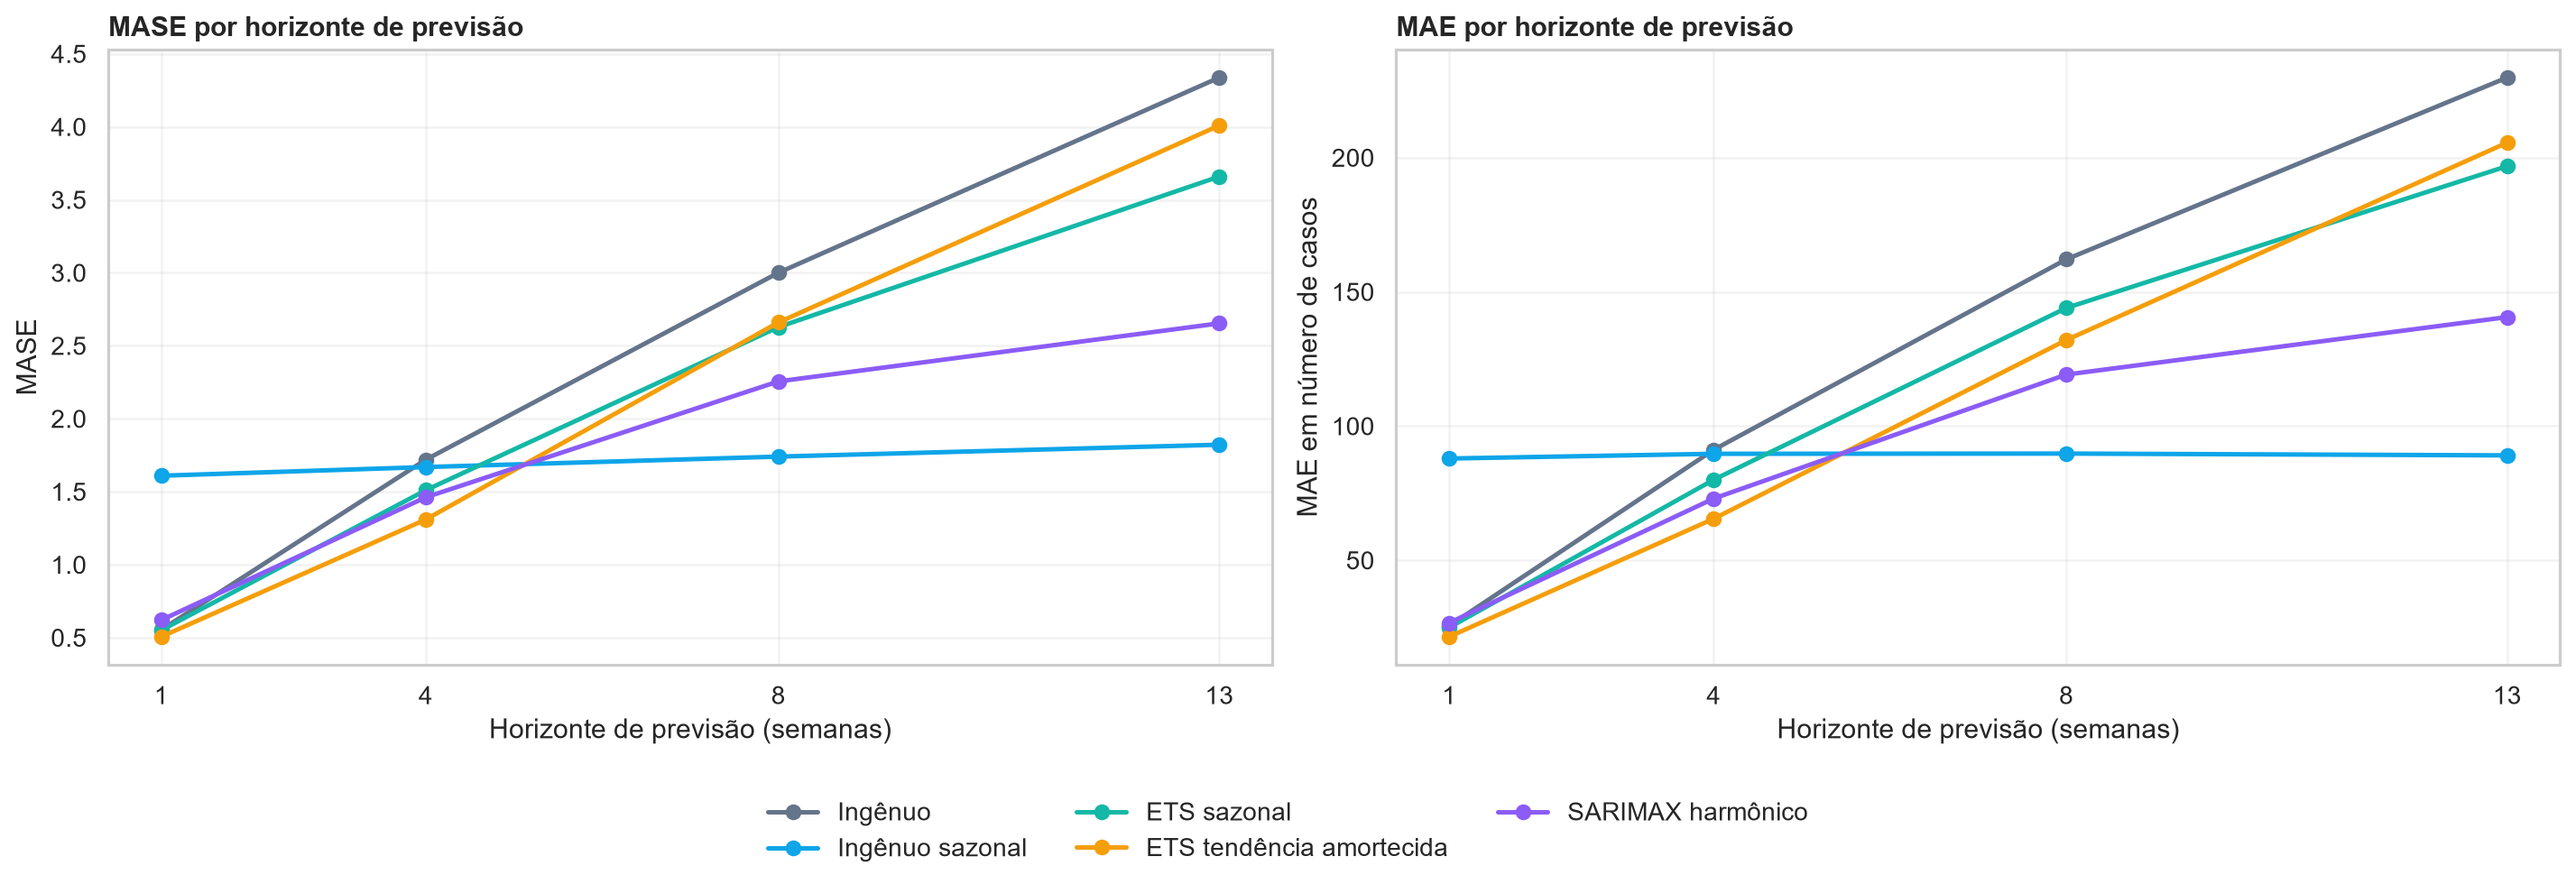
\includegraphics[width=\textwidth]{etapa_26_comparacao_modelos_nao_hierarquicos/comparacao_modelos_nao_hierarquicos.png}
\caption{MASE and MAE by horizon for the eligible non-hierarchical models.}\label{fig:nh}
\end{figure}

The best model depends on the horizon. Damped ETS wins at 1 and 4 weeks, when the recent level carries most of the information. At 8 and 13 weeks the error of every adaptive model grows almost linearly, while the seasonal naive stays flat around MASE 1.7--1.8: repeating last season is the most robust long-range statement. The SARIMAX harmonic model was stable but never best.

For the 27 states, the naive model was best at 1 and 4 weeks (mean MASE 1.145 and 2.285) and the seasonal naive at 8 and 13 weeks (2.990 and 3.122). For intermittent series, carrying forward the last count is hard to beat in the very short term.

\subsection{Incoherence of independent forecasts}
Independent forecasts do not sum. With the first base set, the mean absolute gap between the national forecast and the sum of state forecasts was 253 cases at $h=1$ and 334 at $h=4$. Base V2 reduced it to 53 and 166 cases, respectively (Figure~\ref{fig:inc}), but coherence still held in 0\% of the national comparisons at short horizons. Reconciliation is therefore necessary, not cosmetic.

\begin{figure}[H]
\centering
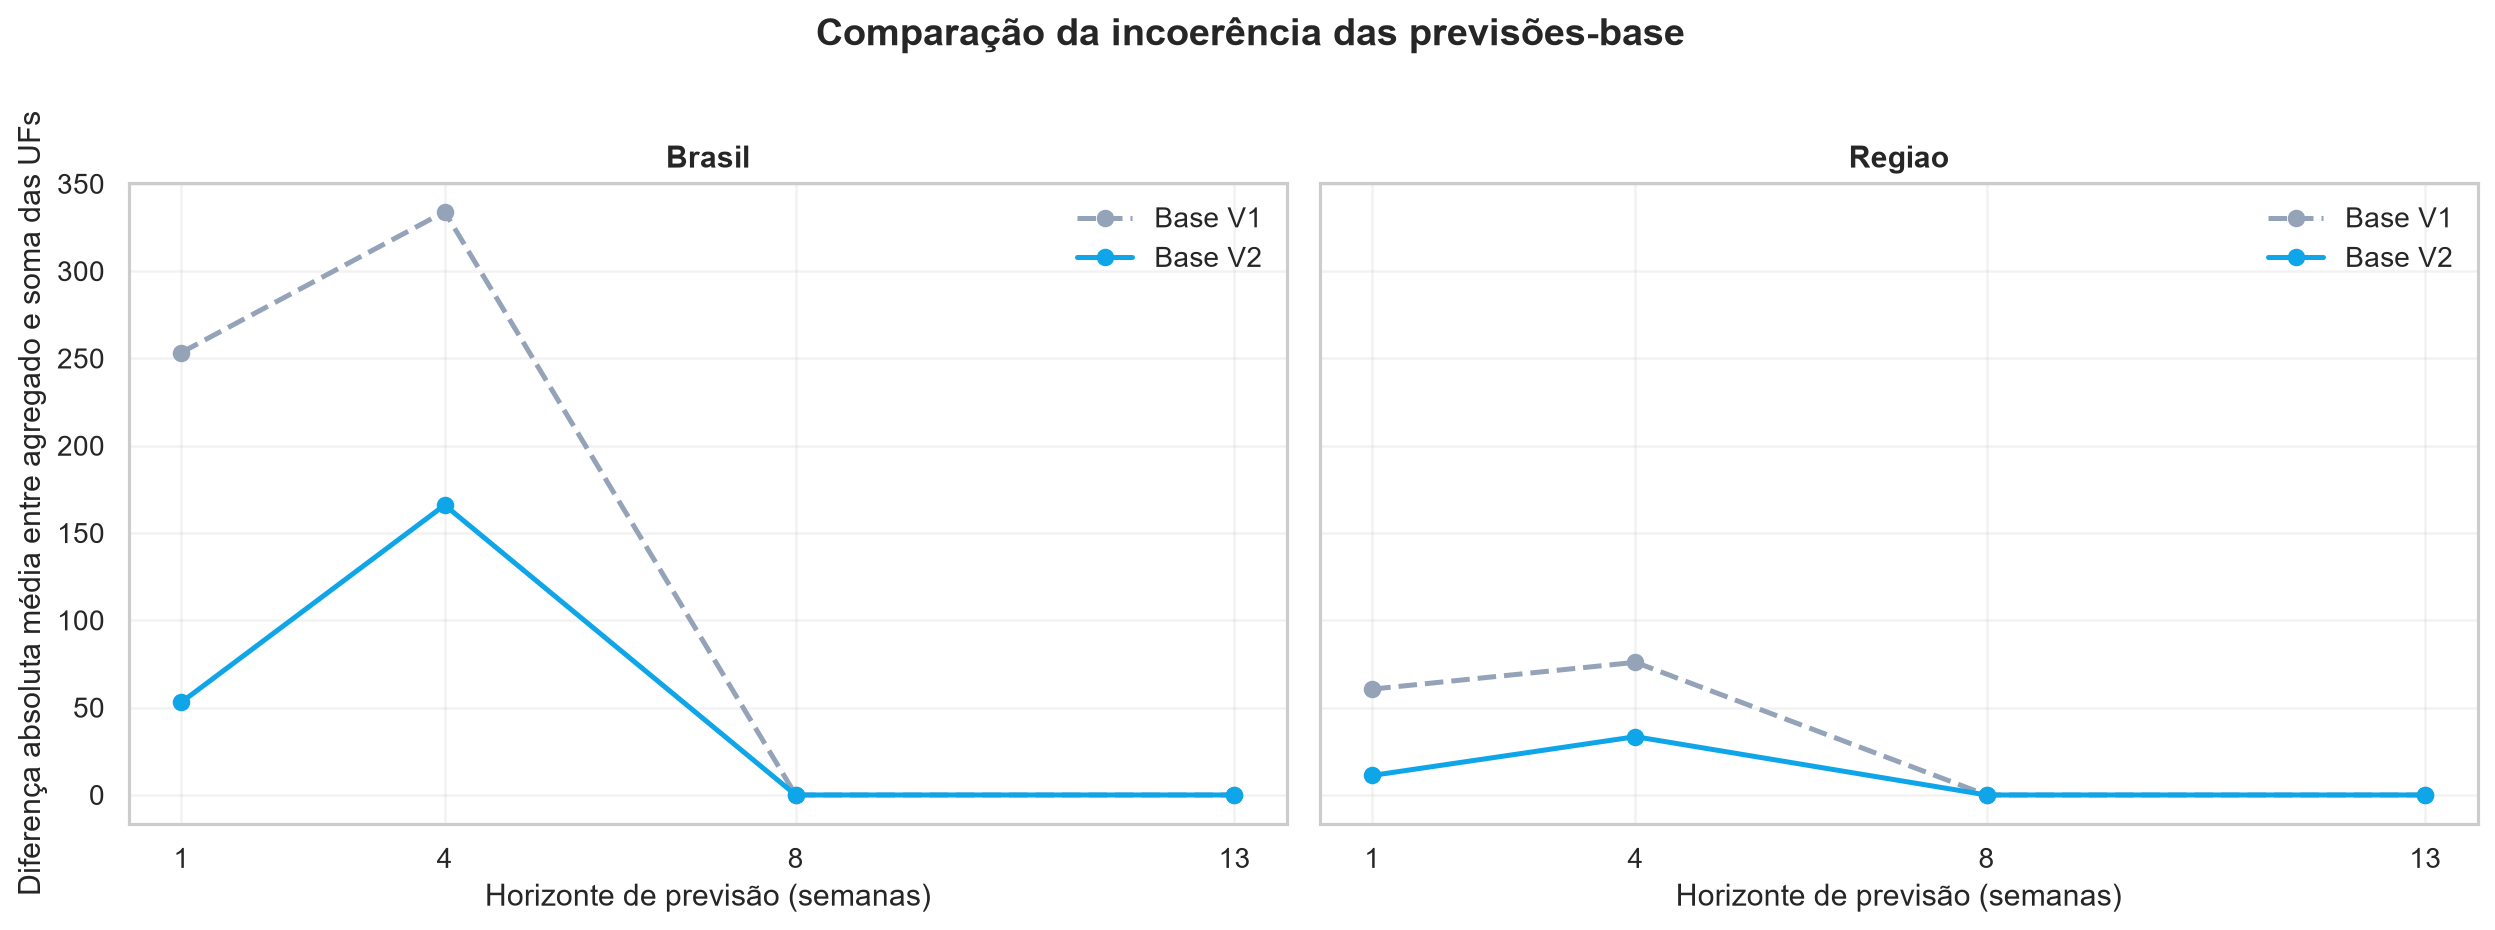
\includegraphics[width=0.95\textwidth]{etapa_30_previsoes_base_hierarquicas_v2/comparacao_incoerencia_base_v1_v2.png}
\caption{Aggregation gap of base forecast sets V1 and V2.}\label{fig:inc}
\end{figure}

\subsection{Hierarchical comparison}
All reconciliation strategies achieved coherence up to numerical precision (maximum gap $8.6\times10^{-11}$ for non-negative MinT). Coherence alone, however, did not decide the choice. Table~\ref{tab:neg} shows that structural WLS and unconstrained MinT-OAS produced a material number of negative state and regional counts at short horizons, which are not acceptable for hospitalization counts. Non-negative MinT produced none, and all 232 optimizations converged.

\begin{table}[H]
\centering\small
\caption{Number of negative forecasts by method (states: 1{,}566 forecasts per horizon; regions: 290).}\label{tab:neg}
\begin{tabular}{lcccc}
\toprule
Method & UF $h=1$ & UF $h=4$ & Region $h=1$ & Region $h=4$ \\
\midrule
Structural WLS & 248 & 316 & 9 & 17 \\
MinT-OAS (unconstrained) & 269 & 312 & 5 & 18 \\
Non-negative MinT & 0 & 0 & 0 & 0 \\
Bottom-up, top-down, Base V2 & 0 & 0 & 0 & 0 \\
\bottomrule
\end{tabular}
\end{table}

\begin{figure}[H]
\centering
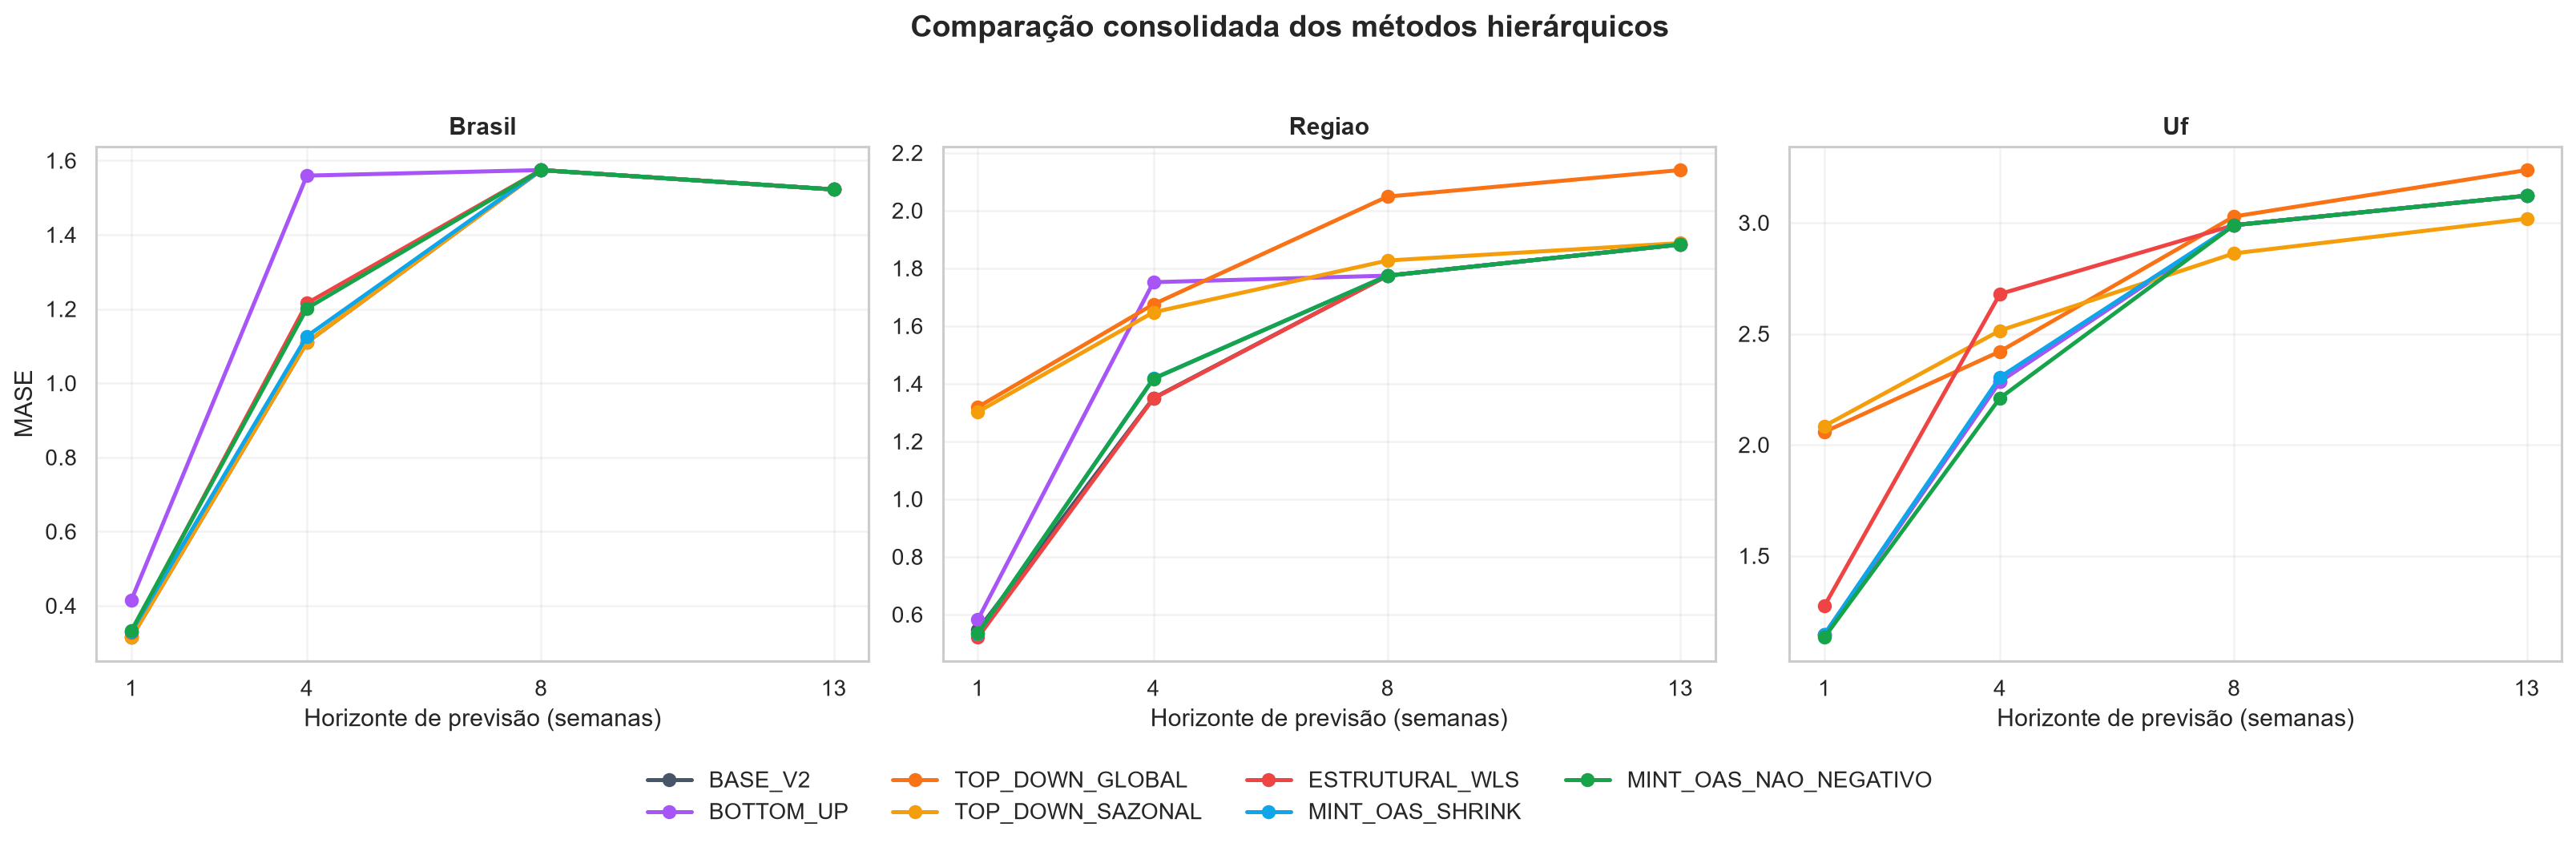
\includegraphics[width=\textwidth]{etapa_37_comparacao_final_hierarquica/comparacao_mase_metodos_hierarquicos.png}
\caption{MASE by horizon and hierarchical level for all strategies.}\label{fig:hier}
\end{figure}

Figure~\ref{fig:hier} and Table~\ref{tab:hier} summarize accuracy. Bottom-up degrades the aggregates (national MASE 0.415 vs.\ 0.315 at $h=1$) and top-down degrades the regions (MASE above 1.3 at $h=1$). Non-negative MinT improves the states at both short horizons and the regions at $h=1$, at the cost of a small loss for Brazil and for the regions at $h=4$. At 8 and 13 weeks all methods coincide with Base V2, which is already coherent.

\begin{table}[H]
\centering\small
\caption{Average MASE: Base V2 (independent) vs.\ non-negative MinT.}\label{tab:hier}
\begin{tabular}{llccl}
\toprule
Level & Horizon & Base V2 & NN-MinT & Reading \\
\midrule
Brazil & 1 & \textbf{0.315} & 0.332 & Base V2 better \\
Brazil & 4 & \textbf{1.110} & 1.202 & Base V2 better \\
Region & 1 & 0.545 & \textbf{0.534} & MinT slightly better \\
Region & 4 & \textbf{1.351} & 1.417 & Base V2 better \\
State  & 1 & 1.145 & \textbf{1.133} & MinT better \\
State  & 4 & 2.285 & \textbf{2.211} & MinT better \\
\bottomrule
\end{tabular}
\end{table}

There is no universal winner. The trade-off is explicit: reconciliation moves information from the aggregates to the sparse states, improving the level where forecasts are hardest, and in exchange accepts a small loss at the national level.

\subsection{Final forecasting policy}
\begin{table}[H]
\centering\small
\caption{Recommended policy by horizon.}\label{tab:policy}
\begin{tabular}{lll}
\toprule
Horizon & Forecast & Reason \\
\midrule
1 week & Non-negative MinT & Coherent, non-negative, better for states \\
4 weeks & Non-negative MinT & Same trade-off \\
8 weeks & Seasonal naive (Base V2) & Already coherent; no gain from reconciliation \\
13 weeks & Seasonal naive (Base V2) & Same argument \\
\bottomrule
\end{tabular}
\end{table}

If the only need is an isolated short-term national number, the direct Base V2 forecast has lower error. When states, regions and Brazil must be reported together, the policy in Table~\ref{tab:policy} is the most defensible choice.

%=====================================================================
\section{Operational Forecast and Uncertainty}\label{sec:op}

After validation was closed, the policy was applied to the last mature origin (19/07/2026), producing 132 forecasts (33 nodes $\times$ 4 horizons) for 26/07/2026 to 18/10/2026. Empirical intervals were derived from the policy's historical residuals over the 58 origins.

\begin{table}[H]
\centering\small
\caption{Operational forecast for Brazil with empirical intervals.}\label{tab:op}
\begin{tabular}{lccc}
\toprule
Horizon & Point forecast & 80\% band & 95\% band \\
\midrule
1 week & 751 & 668--829 & 606--892 \\
4 weeks & 556 & 268--914 & 0--1{,}097 \\
8 weeks & 187 & 0--693 & 0--1{,}267 \\
13 weeks & 83 & 0--569 & 0--1{,}126 \\
\bottomrule
\end{tabular}
\end{table}

Leave-one-out coverage was 76.9--78.4\% for the nominal 80\% bands and 89.7--93.1\% for the 95\% bands: close to, but below, nominal. The bands are therefore practical references, not formal probabilistic guarantees, and they are marginal (state, regional and national bounds do not sum, although the point forecasts do).

A plausibility check flagged that, at this origin, reconciliation shifted the national forecast by 129.2 cases at $h=1$ and 551.0 at $h=4$, well above the historical range of adjustments. This reflects an unusual disagreement between the national ETS and the persistence of the state series at that point of the season, not a coding error. The rule was not changed after seeing the result (that would be post-hoc selection); instead, the forecast is reported as a \emph{reconciled scenario under high disagreement}.

%=====================================================================
\section{Limitations}
\begin{enumerate}\setlength\itemsep{0pt}
\item The series counts notified, confirmed hospitalizations, not all RSV infections; testing coverage varies across years.
\item Changes in testing and reporting, especially in 2020--2021, affect comparability between seasons; the MinT covariance is calibrated across this regime change.
\item Model and policy selection used the same 58 validation origins; a truly independent future evaluation is still pending.
\item Horizons of 8 and 13 weeks carry wide uncertainty and should support scenarios, not exact figures.
\item Reporting delay was handled by excluding immature weeks, not by nowcasting them.
\end{enumerate}

%=====================================================================
\section{Conclusion}\label{sec:conc}

Starting from public microdata and a fully traceable pipeline, this study built a weekly forecasting chain for RSV-associated SARI hospitalizations in children under two at three geographic levels. The central methodological finding is that no single model should be sought: performance depends on the horizon, the geographic level and the intended use. Damped ETS is the best short-term model for dense aggregate series, the seasonal naive remains the most robust option at 8 and 13 weeks, and naive persistence is hard to beat for intermittent states.

Hierarchical reconciliation is needed to publish consistent numbers, but coherence is not enough: unconstrained MinT and WLS generate negative counts, and post-hoc truncation would break coherence. Imposing non-negativity inside the MinT optimization solves both problems and improves state-level accuracy, at a small and explicit cost at the national level. The resulting policy delivers a single, coherent and feasible territorial view, with uncertainty and plausibility warnings attached.

The natural next step is not to fit yet another model on the same origins, but to apply the frozen policy to future mature weeks and evaluate it on an independent window, possibly combined with a nowcasting layer for reporting delays.

\end{document}
